\section{Model2DRigid\-Multi  Class Reference}
\label{classModel2DRigidMulti}\index{Model2DRigidMulti@{Model2DRigid\-Multi}}
A collection of free-floating bodies in a 2D world. 


{\tt \#include $<$model2d.h$>$}

Inheritance diagram for Model2DRigid\-Multi::\begin{figure}[H]
\begin{center}
\leavevmode
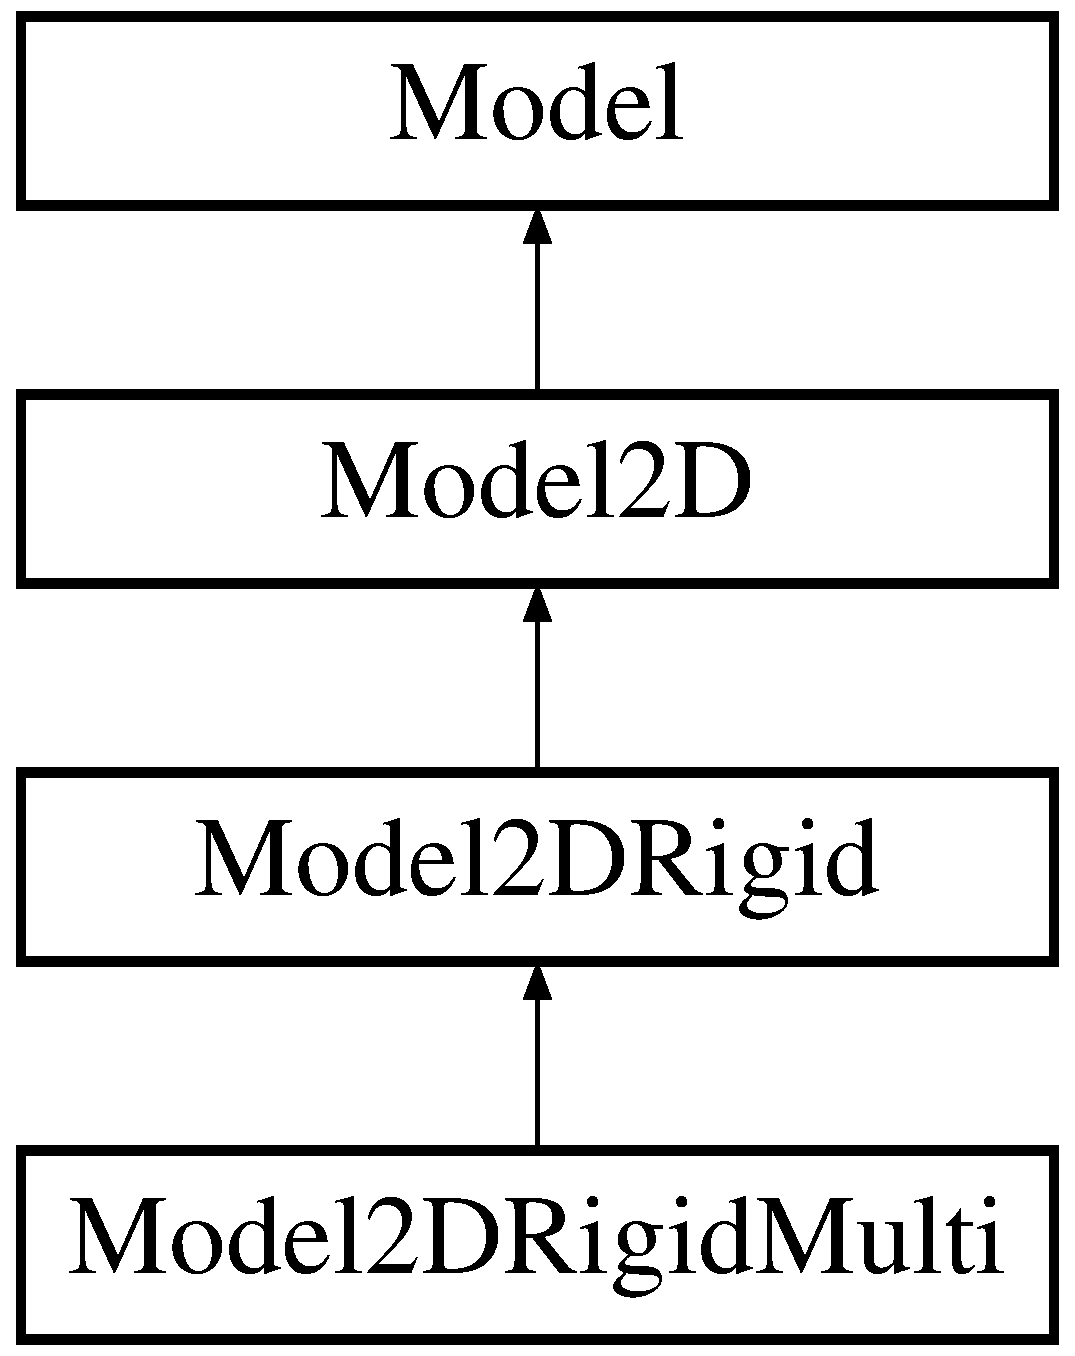
\includegraphics[height=4cm]{classModel2DRigidMulti}
\end{center}
\end{figure}
\subsection*{Public Methods}
\begin{CompactItemize}
\item 
{\bf Model2DRigid\-Multi} (string path)
\item 
virtual {\bf $\sim$Model2DRigid\-Multi} ()
\item 
virtual double {\bf Metric} (const {\bf MSLVector} \&x1, const {\bf MSLVector} \&x2)
\begin{CompactList}\small\item\em A distance metric, which is Euclidean in the base class.\item\end{CompactList}\item 
virtual {\bf MSLVector} {\bf State\-To\-Configuration} (const {\bf MSLVector} \&{\bf x})
\begin{CompactList}\small\item\em A method that converts a {\bf Model} {\rm (p.\,\pageref{classModel})} state in to a {\bf Geom} {\rm (p.\,\pageref{classGeom})} configuration.\item\end{CompactList}\item 
virtual {\bf MSLVector} {\bf Linear\-Interpolate} (const {\bf MSLVector} \&x1, const {\bf MSLVector} \&x2, const double \&a)
\begin{CompactList}\small\item\em Linearly interpolate two state while respecting topology.\item\end{CompactList}\item 
virtual {\bf MSLVector} {\bf State\-Difference} (const {\bf MSLVector} \&x1, const {\bf MSLVector} \&x2)
\begin{CompactList}\small\item\em Compute a {\bf MSLVector} {\rm (p.\,\pageref{classMSLVector})} based on x2-x1. In R$^\wedge$n, the states are simply subtracted to make the {\bf MSLVector} {\rm (p.\,\pageref{classMSLVector})}. This method exists to make things work correctly for other state-space topologies.\item\end{CompactList}\item 
virtual {\bf MSLVector} {\bf Integrate} (const {\bf MSLVector} \&{\bf x}, const {\bf MSLVector} \&u, const double \&h)
\begin{CompactList}\small\item\em Perform integration from state x, using input u, over time step h.\item\end{CompactList}\end{CompactItemize}
\subsection*{Public Attributes}
\begin{CompactItemize}
\item 
int {\bf Num\-Bodies}
\begin{CompactList}\small\item\em Number of independent rigid bodies.\item\end{CompactList}\end{CompactItemize}


\subsection{Detailed Description}
A collection of free-floating bodies in a 2D world.



\subsection{Constructor \& Destructor Documentation}
\index{Model2DRigidMulti@{Model2DRigid\-Multi}!Model2DRigidMulti@{Model2DRigidMulti}}
\index{Model2DRigidMulti@{Model2DRigidMulti}!Model2DRigidMulti@{Model2DRigid\-Multi}}
\subsubsection{\setlength{\rightskip}{0pt plus 5cm}Model2DRigid\-Multi::Model2DRigid\-Multi (string {\em path})}\label{classModel2DRigidMulti_a0}


\index{Model2DRigidMulti@{Model2DRigid\-Multi}!~Model2DRigidMulti@{$\sim$Model2DRigidMulti}}
\index{~Model2DRigidMulti@{$\sim$Model2DRigidMulti}!Model2DRigidMulti@{Model2DRigid\-Multi}}
\subsubsection{\setlength{\rightskip}{0pt plus 5cm}virtual Model2DRigid\-Multi::$\sim$Model2DRigid\-Multi ()\hspace{0.3cm}{\tt  [inline, virtual]}}\label{classModel2DRigidMulti_a1}




\subsection{Member Function Documentation}
\index{Model2DRigidMulti@{Model2DRigid\-Multi}!Integrate@{Integrate}}
\index{Integrate@{Integrate}!Model2DRigidMulti@{Model2DRigid\-Multi}}
\subsubsection{\setlength{\rightskip}{0pt plus 5cm}{\bf MSLVector} Model2DRigid\-Multi::Integrate (const {\bf MSLVector} \& {\em x}, const {\bf MSLVector} \& {\em u}, const double \& {\em h})\hspace{0.3cm}{\tt  [virtual]}}\label{classModel2DRigidMulti_a6}


Perform integration from state x, using input u, over time step h.



Reimplemented from {\bf Model2DRigid} {\rm (p.\,\pageref{classModel2DRigid_a2})}.\index{Model2DRigidMulti@{Model2DRigid\-Multi}!LinearInterpolate@{LinearInterpolate}}
\index{LinearInterpolate@{LinearInterpolate}!Model2DRigidMulti@{Model2DRigid\-Multi}}
\subsubsection{\setlength{\rightskip}{0pt plus 5cm}{\bf MSLVector} Model2DRigid\-Multi::Linear\-Interpolate (const {\bf MSLVector} \& {\em x1}, const {\bf MSLVector} \& {\em x2}, const double \& {\em a})\hspace{0.3cm}{\tt  [virtual]}}\label{classModel2DRigidMulti_a4}


Linearly interpolate two state while respecting topology.

If a=0, then x1 is returned; if a=1, then x2 is returned. All intermediate values of \$a $\backslash$in [0,1]\$ yield intermediate states. This method is defined by {\bf Model} {\rm (p.\,\pageref{classModel})}. 

Reimplemented from {\bf Model2DRigid} {\rm (p.\,\pageref{classModel2DRigid_a4})}.\index{Model2DRigidMulti@{Model2DRigid\-Multi}!Metric@{Metric}}
\index{Metric@{Metric}!Model2DRigidMulti@{Model2DRigid\-Multi}}
\subsubsection{\setlength{\rightskip}{0pt plus 5cm}double Model2DRigid\-Multi::Metric (const {\bf MSLVector} \& {\em x1}, const {\bf MSLVector} \& {\em x2})\hspace{0.3cm}{\tt  [virtual]}}\label{classModel2DRigidMulti_a2}


A distance metric, which is Euclidean in the base class.



Reimplemented from {\bf Model2DRigid} {\rm (p.\,\pageref{classModel2DRigid_a6})}.\index{Model2DRigidMulti@{Model2DRigid\-Multi}!StateDifference@{StateDifference}}
\index{StateDifference@{StateDifference}!Model2DRigidMulti@{Model2DRigid\-Multi}}
\subsubsection{\setlength{\rightskip}{0pt plus 5cm}{\bf MSLVector} Model2DRigid\-Multi::State\-Difference (const {\bf MSLVector} \& {\em x1}, const {\bf MSLVector} \& {\em x2})\hspace{0.3cm}{\tt  [virtual]}}\label{classModel2DRigidMulti_a5}


Compute a {\bf MSLVector} {\rm (p.\,\pageref{classMSLVector})} based on x2-x1. In R$^\wedge$n, the states are simply subtracted to make the {\bf MSLVector} {\rm (p.\,\pageref{classMSLVector})}. This method exists to make things work correctly for other state-space topologies.



Reimplemented from {\bf Model2DRigid} {\rm (p.\,\pageref{classModel2DRigid_a5})}.\index{Model2DRigidMulti@{Model2DRigid\-Multi}!StateToConfiguration@{StateToConfiguration}}
\index{StateToConfiguration@{StateToConfiguration}!Model2DRigidMulti@{Model2DRigid\-Multi}}
\subsubsection{\setlength{\rightskip}{0pt plus 5cm}{\bf MSLVector} Model2DRigid\-Multi::State\-To\-Configuration (const {\bf MSLVector} \& {\em x})\hspace{0.3cm}{\tt  [virtual]}}\label{classModel2DRigidMulti_a3}


A method that converts a {\bf Model} {\rm (p.\,\pageref{classModel})} state in to a {\bf Geom} {\rm (p.\,\pageref{classGeom})} configuration.



Reimplemented from {\bf Model2DRigid} {\rm (p.\,\pageref{classModel2DRigid_a7})}.

\subsection{Member Data Documentation}
\index{Model2DRigidMulti@{Model2DRigid\-Multi}!NumBodies@{NumBodies}}
\index{NumBodies@{NumBodies}!Model2DRigidMulti@{Model2DRigid\-Multi}}
\subsubsection{\setlength{\rightskip}{0pt plus 5cm}int Model2DRigid\-Multi::Num\-Bodies}\label{classModel2DRigidMulti_m0}


Number of independent rigid bodies.



The documentation for this class was generated from the following files:\begin{CompactItemize}
\item 
{\bf model2d.h}\item 
{\bf model2d.C}\end{CompactItemize}
